\documentclass[12pt]{report}

% UCSC Thesis Formatting Requirements
% - Left margin: 1.5" minimum
% - Other margins: 1.25" minimum
% - No headers allowed
% - Page numbers: centered bottom, 3/4" from bottom edge

\usepackage[
    left=1.5in,
    right=1.25in,
    top=1.25in,
    bottom=1.25in,
    footskip=0.5in
]{geometry}

\usepackage{setspace}
\usepackage{titlesec}
\usepackage{tocloft}
\usepackage[pageanchor=true]{hyperref}
\AtBeginDocument{\hypersetup{pageanchor=false}}
\usepackage{graphicx}
\usepackage{url}
\usepackage{natbib}
\usepackage{mathptmx}  % Times New Roman (UCSC guideline: 12pt Times New Roman)
\usepackage{fancyhdr}
\usepackage{amsmath}
% \usepackage{amssymb}  % removed: not used, and rsfs font missing from TeX Live
\usepackage{booktabs}
\usepackage{caption}   % \captionof for non-floating figures
\usepackage{float}     % [H] placement specifier for exact figure positioning

% Remove headers, center page numbers at bottom
\pagestyle{fancy}
\fancyhf{}
\renewcommand{\headrulewidth}{0pt}
\fancyfoot[C]{\thepage}
\fancypagestyle{plain}{\fancyhf{}\fancyfoot[C]{\thepage}\renewcommand{\headrulewidth}{0pt}}

% Double spacing for main text
\doublespacing

% Argument reference command
\newcommand{\argref}[1]{\textbf{#1}}

% Metadata
\newcommand{\thesistitle}{Saturn: Zero-Configuration AI Service Discovery}
\newcommand{\authorname}{Joseph Perrello}
\newcommand{\degreename}{Master of Science}
\newcommand{\departmentname}{Computer Science}
\newcommand{\graduationmonth}{March}
\newcommand{\graduationyear}{2026}
\newcommand{\committeechair}{Ram Sundara Raman}
\newcommand{\committeemembertwo}{Adam Smith}

\begin{document}

% ============================================================
% TITLE PAGE (page i, number NOT displayed)
% ============================================================
\thispagestyle{empty}
\begin{center}
    \textbf{UNIVERSITY OF CALIFORNIA}\\
    \textbf{SANTA CRUZ}\\
    \vspace{0.5in}
    \textbf{\MakeUppercase{\thesistitle}}\\
    \vspace{0.5in}
    A thesis submitted in partial satisfaction\\
    of the requirements for the degree of\\
    \vspace{0.25in}
    \textbf{\MakeUppercase{\degreename}}\\
    \vspace{0.25in}
    in\\
    \vspace{0.25in}
    \textbf{\MakeUppercase{\departmentname}}\\
    \vspace{0.25in}
    by\\
    \vspace{0.25in}
    \textbf{\authorname}\\
    \vspace{0.5in}
    \graduationmonth\ \graduationyear
\end{center}
\newpage

% ============================================================
% APPROVAL PAGE (page ii, number NOT displayed)
% ============================================================
\thispagestyle{empty}
\begin{center}
    \vspace*{1in}
    \begin{flushleft}
    \hspace{3in} The Thesis of \authorname\\
    \hspace{3in} is approved:\\
    \vspace{0.5in}
    \hspace{3in} \rule{2.5in}{0.4pt}\\
    \hspace{3in} \committeemembertwo\\
    \vspace{0.5in}
    \hspace{3in} \rule{2.5in}{0.4pt}\\
    \hspace{3in} \committeechair\\
    \vspace{0.5in}
    \hspace{3in} \rule{2.5in}{0.4pt}\\
    \hspace{3in} Nikos Tziavelis
    \end{flushleft}
\end{center}
\newpage

% ============================================================
% COPYRIGHT PAGE (page ii, number NOT displayed)
% ============================================================
\thispagestyle{empty}
\vspace*{\fill}
\begin{center}
    Copyright \textcopyright\ by\\
    \authorname\\
    \graduationyear
\end{center}
\vspace*{\fill}
\newpage

% ============================================================
% PRELIMINARY PAGES (roman numerals starting at iii)
% ============================================================
\hypersetup{pageanchor=true}
\pagenumbering{roman}
\setcounter{page}{3}

% Table of Contents
\tableofcontents
\newpage

% List of Figures
\listoffigures
\addcontentsline{toc}{chapter}{List of Figures}
\newpage

% List of Tables
\listoftables
\addcontentsline{toc}{chapter}{List of Tables}
\newpage

% ============================================================
% ABSTRACT (not a \chapter heading)
% ============================================================
{
\phantomsection
\addcontentsline{toc}{chapter}{Abstract}
\begin{center}
    \textbf{Abstract}\\
    \vspace{0.25in}
    \thesistitle\\
    \vspace{0.15in}
    \authorname
\end{center}
\vspace{0.5in}

Generative AI services often gate access behind per-user subscriptions, API keys, and manual endpoint configuration. These are barriers that often scale with the number of users and applications on a network.
Saturn, the central contribution of my thesis, provisions AI the way printers and speakers already provision themselves: through Multicast DNS (mDNS) and DNS-based Service Discovery (DNS-SD), network protocols that ship on every major operating system. With Saturn, AI endpoints register under the service type \texttt{\_saturn.\_tcp.local.} and every device on the network discovers them without accounts, credentials, or configuration files.
This thesis contributes the Saturn protocol specification, six reference implementations across four languages, and an on-device deployment on a consumer-grade wireless router. 
}

\newpage

% ============================================================
% GENERATIVE AI ACKNOWLEDGEMENT
% ============================================================
\chapter*{Generative AI Acknowledgement}
\addcontentsline{toc}{chapter}{Generative AI Acknowledgement}

The completion of this thesis excluding Appendix A and \textit{this} acknowledgement would not have been possible without the use of Anthropic's Claude series of LLMs (Opus 4.6, Sonnet 4.5, and Haiku 4.5)\footnote{\url{https://www.anthropic.com/system-cards}} that I (Joey Perrello) obtained while working with Anthropic's coding agent Claude Code.\footnote{\url{https://code.claude.com/docs/en/overview}}  This acknowledgement exists because I (and my advisors, Adam and Ram) believe there should be full disclosure of generative AI when used in the creation of academic work, as some readers may be morally opposed to generative AI. Previous academic work went uncredited into the training of the models, so it is the responsibility of academics to attempt to show respect to those who contributed before by acknowledging use of LLMs. My advisors recommended this thesis' use of generative AI under the conditions that there was a \textit{human-written} acknowledgement and an appendix entry detailing how the system works. The resulting system is an agent-assisted research flow that is systematic and comprehensive, and an integral aspect of this thesis' creation. I originally intended Saturn, the protocol discussed in this thesis, to be a Master's project, where the guidelines for completion were more relaxed than a Master's thesis. I decided at the beginning of the academic quarter to transition to a thesis. During this time I became inspired by the agent driven development work of Geoffrey Huntley (of Ralph loops\footnote{\url{https://ghuntley.com/ralph/}}), Dexter Horthy (of 12-factor agents\footnote{\url{https://github.com/humanlayer/12-factor-agents}}), and Steve Yegge (of Gas Town\footnote{\url{https://steve-yegge.medium.com/welcome-to-gas-town-4f25ee16dd04}}).  This inspiration spawned the idea of an academic research assistant with the same knowledge and comprehension of Saturn as my own. However, this system ended up requiring the same level of attention and focus as Saturn, with similar levels of complexity. The system and all use cases of LLMs in this thesis is described in Appendix A. The initial design of Saturn, the ideas expressed in this paper, and the final copy are reflections of my own ideas and beliefs.

\newpage

% ============================================================
% MAIN TEXT (Arabic numerals starting at 1)
% ============================================================
\pagenumbering{arabic}
\setcounter{page}{1}

\chapter{Introduction}
\label{ch:introduction}

As a graduate student paying one-hundred dollars per month across several AI services, I watched peers go without AI tools that had become part of my daily workflow. The technology itself is expensive to run, and the delivery model is not designed for easy access. Syed et al.~\cite{syed2025aiaas} documented this systems problem: the dominant pattern requires users to create an account, supply payment credentials, obtain an API key, and manually configure that key into every application. A student seeking three capabilities from three providers must manage three subscriptions, three keys, and three billing relationships. These barriers create measurable disparities; Bassignana et al.~\cite{bassignana2025aigap} and Gabriel~\cite{gabriel2024educational} showed that users from lower socioeconomic backgrounds interact with language technologies less frequently and derive less benefit. I wanted to provision AI services to everyone on my campus the way universities already provision other shared resources. A student who joins the eduroam network gains access to printers, file shares, and licensed software without creating accounts or entering credentials. There is no zero-configuration protocol advertises, discovers, and connects to AI service endpoints.

I define \emph{Saturn} as the process of advertising AI service API endpoints via mDNS packets on a local network, discovering those endpoints through standard DNS-SD queries, and transferring data between client and service using the discovered connection parameters. A \emph{Saturn service} is any AI endpoint advertised via the \texttt{\_saturn.\_tcp.\allowbreak{}local.} service type. Saturn extends the existing TXT record mechanism to carry endpoint URLs, API types, and authentication credentials without protocol modifications. I created six implementations that consume the same service type with no shared discovery code, no bridging layer, and no user configuration. Python, Rust, and TypeScript clients each resolve Saturn independently. This cross-platform interoperability establishes the first claim (\argref{C1}): zero-configuration network protocols can provision AI services without end-user configuration.

The second claim addresses whether this model actually reduces work (\argref{C2}). A cognitive walkthrough comparing Saturn against traditional per-user API provisioning shows that Saturn reduces combined configuration steps by 53\%, with application developers experiencing a 79\% reduction. The gain is not free: Saturn centralizes all setup in one administrator, who takes on more steps than a single traditional user would. But that one operator replaces the configuration burden of every consumer on the network. 

Zero-configuration access requires a security trade-off. Saturn broadcasts service metadata to every device on the network, and requiring per-device authentication would reintroduce the credential burden the protocol exists to eliminate. I chose to document and bound the exposure instead. The mDNS threat models that Kaiser and Waldvogel~\cite{kaiser2014privacy} established map the attack surface, and ephemeral credentials with ten-minute expiry windows limit what a compromised key can do. I analyze these trade-offs against the static API key model Saturn displaces in the security section of Chapter~\ref{ch:discussion}.

Together, these contributions argue that AI access can and should be provisioned at the network level. Saturn demonstrates the technical feasibility of this model, quantifies its usability benefits, and maps the security surface that any future deployment must address.


\chapter{Background}
\label{ch:background}

\section{Multicast DNS and DNS-Based Service Discovery}
\label{sec:mdns-dnssd}

I selected mDNS/DNS-SD because it implements the exact discovery patterns for networked peripherals I required for distributed AI services. Multicast DNS (mDNS), as defined in RFC 6762 \cite{rfc6762}, enables peer-to-peer name resolution on a local network by querying the multicast address \texttt{224.0.0.251} (or \texttt{ff02::fb} for IPv6) over port 5353. By utilizing the \texttt{.local} top-level domain, mDNS allows devices to resolve hostnames without reliance on external DNS infrastructure, fulfilling the "zero-configuration" vision described by Guttman \cite{guttman2001zeroconf}. DNS-based Service Discovery (DNS-SD), specified in RFC 6763 \cite{rfc6763}, layers structured advertisement on top of mDNS through three DNS record types: PTR records enumerate service instances, SRV records provide the hostname and port, and TXT records carry key-value metadata. 

The viability of Saturn relies on the broad cross-platform support of these protocols. Apple's Bonjour \cite{bonjour}, released in 2002, ships natively with macOS and iOS and is available as a Windows service, while Avahi \cite{avahi} serves as the default mDNS daemon on most Linux distributions. As Siddiqui et al. \cite{siddiqui2012zeroconf} confirmed, Avahi and Bonjour interoperate correctly on typical local networks, and Siljanovski et al. \cite{siljanovski2014mdns} demonstrated that mDNS functions even on resource-constrained hardware. Together, these implementations allow Saturn to leverage OS-level discovery without requiring users to install external daemons, maintaining the project's zero-configuration premise.

By leveraging TXT records, Saturn encapsulates structured metadata—including endpoint URLs, API types (such as OpenAI-compatible or Ollama), and authentication credentials—into a single announcement. This effectively automates the manual configuration typically required for AI services. However, this approach necessitates designing around specific mDNS constraints: a 255-byte limit per TXT string, link-local scope restrictions, and the inherent lack of native broadcast security. 

The same broadcast visibility that enables discovery also creates a privacy surface. Kaiser and Waldvogel \cite{kaiser2014privacy} showed that passive eavesdropping on mDNS traffic reveals which services a device offers and consumes, while Könings et al. \cite{konings2013devicenames} found that 59\% of mDNS device names contain the owner's real name. For Saturn, these findings mean that AI endpoint announcements—including ephemeral API keys—are visible to every device on the local network. To mitigate these risks, Chapter \ref{ch:design} details the specific TXT schema and the use of ephemeral keys, while Chapter \ref{ch:discussion} provides a full evaluation of the protocol's performance and security trade-offs at scale.protocol's performance at scale.

\section{Alternative Protocol Analysis}
\label{sec:comparisons}

I evaluated four alternative service discovery protocols against three core requirements: cross-platform support, structured metadata, and zero-infrastructure operation. Among these, NetBIOS \cite{rfc1001} is the least viable, as it lacks structured metadata beyond a 15-character hostname and has been deprecated by Microsoft in favor of mDNS since Windows 10. Similarly, DLNA \cite{dlna2017} is unsuitable because it restricts its scope to media streaming, its consortium dissolved in 2017, and its schema cannot express critical information like API types or authentication tokens.

WS-Discovery \cite{wsdiscovery} and UPnP \cite{upnp2015} offer more robust metadata capabilities but introduce significant overhead. WS-Discovery relies on SOAP/XML messages, where a single probe consumes roughly 1\,KB of XML compared to a 50-byte DNS query; such verbosity makes Saturn beacons impractical for weaker networks. UPnP comes closest to meeting the requirements due to its rich device descriptions and active deployment, yet it bundles unnecessary control features like event subscriptions. Furthermore, security vulnerabilities in UPnP's control surface have led US-CERT to recommend its deactivation, whereas Saturn requires lean discovery without remote-control risks.

The structural insight of the Dynamic Host Configuration Protocol (DHCP) \cite{rfc2131} served as the primary inspiration for Saturn's design. In a DHCP workflow, a device broadcasts a DISCOVER message and receives an OFFER, allowing it to operate without manual user configuration. Saturn adopts this concentration of complexity to eliminate per-user configuration for AI service endpoints. By centralizing the logic within the protocol, one administrator can configure the server while every client benefits automatically, validating the principle of infrastructure-level provisioning. Despite this conceptual alignment, Saturn departs from DHCP in three functional ways that necessitated a new implementation. First, Saturn manages multiple dynamic services as they start and stop, rather than assigning a single static address at network join. Second, Saturn operates entirely in userspace without requiring the privileged access necessary to configure network interfaces. Finally, Saturn communicates via multicast DNS on port 5353 after connectivity is established, rather than operating below the IP layer on UDP port 67. These distinctions ensure that Saturn provides high-level AI service discovery while maintaining the zero-configuration strengths of the DHCP model.

\chapter{Protocol Design}
\label{ch:design}

\section{Design Goals}
\label{sec:design-goals}

Central to the vision of Saturn is the pursuit of zero-configuration consumer access. By ensuring that network connectivity alone grants access to AI services, Saturn removes the traditional barriers of URLs, API keys, and account management. Every protocol decision detailed in this chapter is evaluated against its ability to preserve this property, specifically targeting the elimination of the platform lock-in and per-user key management documented by Syed et al.~\cite{syed2025aiaas}.

\begin{figure}[ht]
\centering
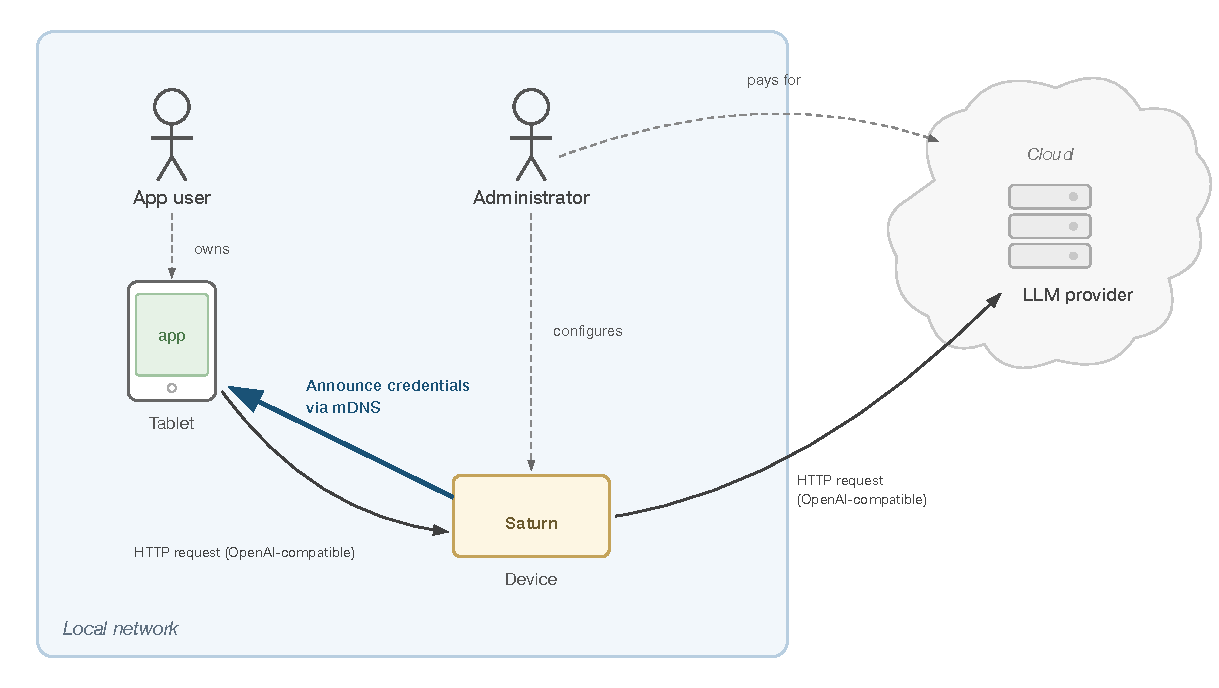
\includegraphics[width=0.85\textwidth]{figures/saturn-network.pdf}
\caption[Overview of Saturn's network architecture.]{Overview of Saturn's network architecture. The Saturn device announces service credentials via mDNS on the local network. Applications discover the service and issue OpenAI-compatible HTTP requests. The administrator configures the device and manages the cloud provider relationship; the app user interacts only with the application.}
\label{fig:saturn-network}
\end{figure}

Saturn must also remain resilient to the volatile landscape of AI inference. To prevent the protocol from locking into a specific backend and ensuring long-term relevance, backend agnosticism is treated as a core requirement. This abstraction allows Saturn to express diverse environments—ranging from local Ollama instances to cloud proxies like OpenRouter through a unified interface. Finally, this high degree of accessibility is balanced against a documented security posture. Rather than ignoring the risks of local credential broadcasting, Saturn’s design explicitly accounts for these trade-offs. As detailed in Section~\ref{sec:security}, the architecture establishes rigorous threat models and mitigations tailored for the trust profiles of homes, offices, and research laboratories.

\section{Audiences}
\label{sec:audiences}

Saturn defines three roles. Three is the minimum decomposition that separates credential management (administrator), integration logic (developer), and usage (end user) into distinct responsibility boundaries. Every design decision identifies which role bears complexity and which roles benefit. Figure~\ref{fig:audiences} summarises each role.

\begin{center}
\fbox{\begin{minipage}{0.9\textwidth}
\begin{singlespace}
\small
\smallskip
\textbf{Administrator.}\quad Deploys and configures Saturn services: selects backends, sets priorities, manages API credentials, and monitors health. The only role that touches configuration files or credentials. In a university department, this is IT staff; in a home, the technically inclined household member. Running Saturn adds one configuration file and one background process---a fixed cost amortized across every other user on the network.

\medskip
\textbf{Application developer.}\quad Integrates Saturn discovery into software. Rather than hard-coding endpoints and requiring users to supply credentials, the developer calls a function like \texttt{discover()} that returns available services with URLs and credentials already populated. No authentication logic, no configuration UI, no billing integration. Chapter~\ref{ch:implementation} details the integration patterns.

\medskip
\textbf{End user.}\quad Interacts with AI-powered applications without awareness that Saturn exists. A student opens a chat application on the campus network, types a question, and receives a response---no API key prompt, no account creation, no settings page. This role performs zero configuration steps.
\smallskip
\end{singlespace}
\end{minipage}}
\captionof{figure}{Saturn's three audience roles and their responsibilities.}
\label{fig:audiences}
\end{center}
\section{Standardizing Endpoint Communication}
\label{sec:standardized-interface}

To ensure seamless interoperability across a landscape of different AI providers, Saturn mandates that every discovered backend adhere to a unified communication protocol. Rather than introducing a proprietary schema, Saturn adopts the OpenAI-compatible REST API as its foundational interface. This grants Saturn immediate compatibility with established backends such as Ollama~\cite{ollama} and OpenRouter~\cite{openrouter}.

To qualify as a valid Saturn \emph{endpoint}, a service must implement a foundational subset of the OpenAI specification, specifically exposing the following three paths:
\begin{itemize}
    \item \texttt{GET /health}: A diagnostic route returning a JSON object to verify service liveness and operational readiness.
    \item \texttt{GET /v1/models}: An enumeration endpoint that provides a list of available models and their metadata in the standardized list-models format.
    \item \texttt{POST /v1/chat/completions}: The primary data exchange route, supporting the full breadth of chat completion requests, including both atomic and multiplexed streaming responses.
\end{itemize}

The adoption of this standard facilitates a "zero-configuration" deployment model: any application designed for OpenAI’s infrastructure can function as a Saturn client, and any compatible backend becomes instantly discoverable. While this introduces a structural dependency on a third-party specification, the stability of the \texttt{/v1/chat/\allowbreak{}completions} interface and its widespread adoption as a \textit{de facto} industry standard mitigate the risks of breaking changes. By prioritizing ubiquitous compatibility over custom extensibility, Saturn minimizes the technical friction typically associated with decentralized service integration.

\section{Service Advertisement}
\label{sec:service-advertisement}
\label{sec:service-type}
\label{sec:txt-schema}

Saturn registers services under the DNS-SD service type \texttt{\_saturn.\_tcp.local.}. The underscore prefix follows DNS-SD naming conventions (RFC~6763~\cite{rfc6763}), the \texttt{\_tcp} transport selector indicates the endpoint communicates over TCP (HTTP), and the \texttt{.local.} domain restricts discovery to the link-local mDNS scope.

Each Saturn service produces the standard DNS-SD record triple (PTR, SRV, TXT) described in Chapter~\ref{ch:background}. Saturn's contribution is the TXT record schema: key-value pairs encoded per RFC~6763 (each pair as a single DNS TXT string, formatted as \texttt{key=value}). Table~\ref{tab:txt-fields} specifies the fields.

\begin{table}[ht]
\centering
\caption{Saturn TXT record fields. Fields marked required must appear in every advertisement.}
\label{tab:txt-fields}
\begin{tabular}{@{}llp{2.8in}@{}}
\toprule
\textbf{Field} & \textbf{Required} & \textbf{Description} \\
\midrule
\texttt{version}           & Yes & Protocol version (currently \texttt{1}) \\
\texttt{api\_type}         & Yes & Backend API format (e.g., \texttt{openai}) \\
\texttt{deployment}        & Yes & One of \texttt{local}, \texttt{cloud}, or \texttt{network} \\
\texttt{priority}          & Yes & Numeric routing preference; lower is preferred \\
\texttt{api\_base}         & Conditional & Base URL of the endpoint. Required when \texttt{deployment=cloud}; for local and network deployments, clients construct the URL from the SRV record's host and port \\
\texttt{ephemeral\_key}    & No  & Current API credential; present only for cloud deployments \\
\texttt{rotation\_interval}& No  & Key rotation period in seconds (default: 300) \\
\texttt{features}          & No  & Comma-separated capability list (e.g., \texttt{chat,vision,tools}) \\
\toprule
\end{tabular}
\end{table}

\label{sec:priorities}
The \texttt{priority} field gives administrators a way to express routing policy without requiring clients to understand that policy. Each beacon advertises a numeric priority, lower numbers indicating higher preference. Clients sort by priority and select the lowest-numbered available service. Consider a lab with a local GPU server and a cloud fallback: the administrator sets the Ollama beacon to priority~1 and the OpenRouter beacon to priority~10. Clients prefer local inference automatically. If the local server goes down, they fall back to the cloud service with no user intervention. The semantics mirror DNS SRV record priority (RFC~6763~\cite{rfc6763}), a convention already familiar to network administrators.

\label{sec:ephemeral-keys}
The \texttt{ephemeral\_key} field addresses a harder problem. Meli et al.~\cite{meli2019secrets} found over 100,000 GitHub repositories containing leaked secrets, 81\% never removed after notification. Static keys fail because every mitigation---detection, rotation, revocation---acts after the damage. Saturn sidesteps this failure class with \emph{ephemeral keys}: time-limited API credentials that a cloud beacon generates, broadcasts in its TXT record, and deletes after expiration. The default lifecycle uses a ten-minute key lifetime and a five-minute rotation interval, creating an overlap window where both current and next key are valid. A key that expires in ten minutes is worthless by the time someone extracts it from a packet capture, commits it to a repository, or pastes it in a chat log. The trade-off is operational: ephemeral keys require the beacon to maintain an active session with the cloud provider's key provisioning API. If the beacon loses connectivity, it cannot rotate keys, and the current key eventually expires without replacement. Section~\ref{sec:security} analyzes this and other failure modes.

DNS-SD imposes a 255-byte limit per TXT string (RFC~6763~\cite{rfc6763}). After the \texttt{ephemeral\_key=} prefix, approximately 240 characters remain for the credential itself. JWT tokens from OpenRouter and DeepInfra fit; full X.509 certificates do not. I chose to carry credentials inline in the TXT record rather than requiring clients to fetch them from an HTTPS bootstrap endpoint, because a bootstrap endpoint would reintroduce the infrastructure dependency Saturn exists to eliminate. The constraint is that credential formats must be compact enough for a single TXT string.

\label{sec:discovery-flow}
With the advertisement defined, the discovery flow replaces the configuration file or environment variable that would otherwise contain an API URL and key. Four steps execute without user interaction:

\begin{enumerate}
    \item \textbf{Browse}: The client queries for PTR records of type \texttt{\_saturn.\_tcp.local.}. All beacons on the local network respond with their instance names.
    \item \textbf{Resolve}: For each instance, the client retrieves the SRV record (hostname, port) and TXT record (metadata).
    \item \textbf{Select}: The client sorts by \texttt{priority} (ascending), optionally filters by \texttt{features} or \texttt{deployment} type, and selects the preferred service.
    \item \textbf{Connect}: For cloud deployments, the client uses \texttt{api\_base} and attaches the \texttt{ephemeral\_key} as a Bearer token. For local and network deployments, it constructs the URL from the SRV record (e.g., \texttt{http://\{host\}:\{port\}/v1}).
\end{enumerate}

\section{Beacons}
\label{sec:beacon-architecture}

In the absence of a centralized registry, Saturn facilitates endpoint discovery through a decentralized \emph{beacon} mechanism. Leveraging the Multicast DNS (mDNS) protocol, a beacon broadcasts critical service metadata—including endpoint URLs, API specifications, priority metrics, and authentication requirements—without intercepting or proxying the underlying API traffic. By strictly bifurcating the discovery layer from the data plane, this architecture ensures that clients establish direct peer-to-peer connections with the advertised services.

Beacons are categorized by their deployment scope. A \emph{local} beacon facilitates service discovery within a shared network namespace or LAN, such as a local LLM instance. Conversely, a \emph{cloud} beacon serves as a bridge to remote environments (e.g., OpenRouter), distributing ephemeral credentials that allow network participants to use administrative accounts without individual credential management. While a proxy-based approach would offer native rate limiting and centralized logging, such features demand hardware resources and observational access that contradict Saturn's core objectives. By delegating usage auditing to external reverse proxies at the endpoint level, Saturn maintains a lean, non-intrusive discovery fabric that eliminates the beacon as a single point of failure or a surveillance chokepoint.

\section{Security}
\label{sec:security}

Saturn deliberately trades enterprise-grade verification for zero-configuration access. Two threat models define the boundaries of that trade-off. The mitigations described here are design-time claims; Chapter~\ref{ch:evaluation} evaluates whether they hold in practice.

\subsection{Threat Model 1: Corporate Data Collection}
\label{sec:threat-corporate}

I do not want companies like OpenAI or Anthropic collecting my prompts, conversation histories, or usage patterns. This is the first threat Saturn addresses: a user's AI interactions flow to a cloud provider who retains, analyzes, or monetizes them.

Saturn addresses this threat concretely: an administrator deploys a local inference server---Ollama with an open-weights model---and sets its priority higher than any cloud beacon. Users on the network route to the local service automatically. Their prompts never leave the LAN. This works because the protocol is backend-agnostic; it does not prescribe what runs behind the endpoint.

The limitation is capacity. Local inference requires hardware that matches or approximates the capability of cloud models. A university department can justify a GPU server; a household typically cannot. When the local model is insufficient and the user falls back to a cloud endpoint, Saturn provides no additional data protection beyond what the cloud provider offers. Saturn enables the administrator to make local inference the default path, but it cannot guarantee that path is always available.

\subsection{Threat Model 2: Untrusted Administrator}
\label{sec:threat-admin}

I do not trust the system administrator of my office or house not to snoop. The sysadmin controls the beacon and could route traffic through a logging proxy, advertise a malicious endpoint, or retain copies of ephemeral keys.

The administrator is, by design, the trusted party, so Saturn provides limited mitigation here. The administrator who runs only a beacon cannot see prompts or responses, because API traffic flows directly from client to endpoint. The administrator sees only the metadata broadcast in TXT records---metadata the administrator created in the first place.

An administrator who controls both the beacon and the endpoint, however, has full access to all traffic. Saturn cannot protect against this scenario without introducing user-level authentication, which would destroy the zero-configuration property. This is the fundamental trade-off the architecture makes: Saturn trusts the network in the same way that connecting to office WiFi trusts the network operator with DNS resolution and IP routing. Ward and Beyer~\cite{ward2014beyondcorp} argued in BeyondCorp that networks should never be trusted; Saturn disagrees for its target environment of homes, offices, and campus labs where the network operator is a known party and the alternative---per-user credential management---creates the access barriers Saturn exists to remove.

\subsection{Broadcast Exposure}
\label{sec:broadcast-exposure}

Any device on the local network can observe Saturn's mDNS announcements---the broadcast exposure that Section~\ref{sec:mdns-dnssd} documented applies here. For local deployments, the exposed information is limited to service existence and location. For cloud deployments, the TXT record also contains an ephemeral API key readable by any network participant.

Two mechanisms bound the financial exposure: the ephemeral key lifecycle described in Section~\ref{sec:ephemeral-keys} limits the exploitation window, and administrators can set spending limits on their cloud provider accounts. These mitigations bound impact rather than eliminate the threat. Deployments requiring stronger guarantees must add network-level access control (e.g., VLAN segmentation or 802.1X authentication) outside Saturn's scope. Kaiser and Waldvogel~\cite{kaiser2014efficient} proposed privacy-preserving extensions to mDNS-SD, a direction Chapter~\ref{ch:discussion} explores.


\chapter{Reference Implementations}
\label{ch:implementation}

Chapter~\ref{ch:design} specified Saturn's protocol---a service type, a TXT record schema, a discovery flow, and a security posture. This chapter describes how I realized that design in code. I built three implementations in sequence under a fixed project timeline, each answering a question the previous one left open: Can Saturn bring AI to an application that has never had it? Can it provision AI at the network infrastructure layer? Can it handle the full complexity of agentic tool calling? All three build on a shared foundation of two packages I wrote. Both packages build on existing dependencies: the Python \texttt{zeroconf} library for mDNS advertisement and Vercel's AI SDK \texttt{ProviderV3} interface with the \texttt{multicast-dns} npm library for TypeScript discovery. On top of these, I built two original packages. The \texttt{saturn-ai} Python package\footnote{\url{https://github.com/jperrello/Saturn/tree/main/saturn}} adds ephemeral credential generation, OpenAI-compatible HTTP endpoints, and proxying to any upstream backend. The \texttt{ai-sdk-provider-saturn} npm package\footnote{\url{https://github.com/jperrello/Saturn/tree/main/ai-sdk-provider-saturn}} adds discovery orchestration, circuit breaking, and failover. These two packages use different mDNS libraries in different languages yet interoperate on the same service type and TXT record schema, supporting argument~\argref{A2}.

\section{VLC Extension: AI in a Non-AI-Native Application}
\label{sec:vlc-implementation}

A protocol that works only inside developer tools would be a weak demonstration of \argref{C1}.
VLC media player --- one of the most widely installed desktop applications --- has never offered AI features.
I chose it precisely for that reason: if Saturn can bring AI into VLC without the user configuring anything, the protocol demonstrates value beyond AI-native contexts.

\subsection{Architecture and Technology Choices}

VLC's extension system accepts only Lua scripts, and its HTTP support is limited to GET requests via \texttt{vlc.stream()}. No POST, no mDNS, no JSON library. These constraints ruled out embedding Saturn discovery directly in the extension.

I built a two-layer architecture.
A Lua extension (\texttt{saturn\_roast.lua}\footnote{\url{https://github.com/jperrello/Saturn/blob/main/vlc_extension/saturn_roast.lua}}, v1.0.0) provides the in-player GUI: a service dropdown, a single ``Roast Me!'' button, and styled HTML output.
I chose the roast variant over the conversational Saturn Chat extension because it better demonstrates the thesis claim: the user clicks one button, receives comedic commentary about their media choices, and never encounters a chat interface or any indication that a language model is involved.
A Python/FastAPI bridge (\texttt{vlc\_discovery\_bridge.py}\footnote{\url{https://github.com/jperrello/Saturn/blob/main/vlc_extension/vlc_discovery_bridge.py}}) runs as a background process, performing mDNS discovery and exposing an OpenAI-compatible REST API on localhost.
The bridge uses macOS's \texttt{dns-sd} CLI for discovery rather than the \texttt{zeroconf} library: a non-technical VLC user should install Saturn by copying a single directory, and bundling \texttt{zeroconf} into a standalone PyInstaller executable would add native dependencies that complicate that goal.

Two trade-offs follow from VLC's constraints.
Because Lua cannot POST, the extension sends request payloads as URL-encoded JSON in GET query parameters, which imposes URL length limits (typically 2,048 characters) on messages.
The bridge also requires a background Python process, adding a launch delay and a second process the user does not see.
I wrote a hand-written recursive descent JSON parser for Lua since VLC provides no JSON library.

I expect this bridge pattern to generalize: any application that can issue HTTP requests to the standard \texttt{/v1/} endpoints can integrate Saturn through a local bridge, though each bridge inherits platform-specific discovery costs and requires a background process.

When a user activates the extension (View $\rightarrow$ Extensions $\rightarrow$ Saturn Roast):

\begin{enumerate}
\item The extension locates the bundled bridge executable and launches it in the background with a \texttt{-{}-port-file} argument.
\item The bridge auto-detects an available port, starts the HTTP server, and writes \texttt{host:port} to the port file.
\item The extension polls the port file, then health-checks the bridge with exponential backoff (seven retries over approximately seven seconds).
\item Once ready, the extension queries \texttt{/services} to populate the service dropdown. The bridge browses \texttt{\_saturn.\_tcp.local.} every ten seconds in a background thread.
\item The user clicks ``Roast Me!'' The extension extracts media context --- title, artist, playback position --- via \texttt{vlc.input.item():metas()}, composes a single request with a system prompt instructing the model to roast the user's media taste, and the bridge proxies the request to the selected Saturn service. The model returns a short comedic response (capped at 200 tokens) with no persistent conversation history.
\end{enumerate}

Figure~\ref{fig:vlc-roast} shows the resulting dialog: the service dropdown, the ``Roast Me!'' button, and styled HTML output displaying the model's comedic commentary about the currently playing media.

\begin{figure}[H]
\centering
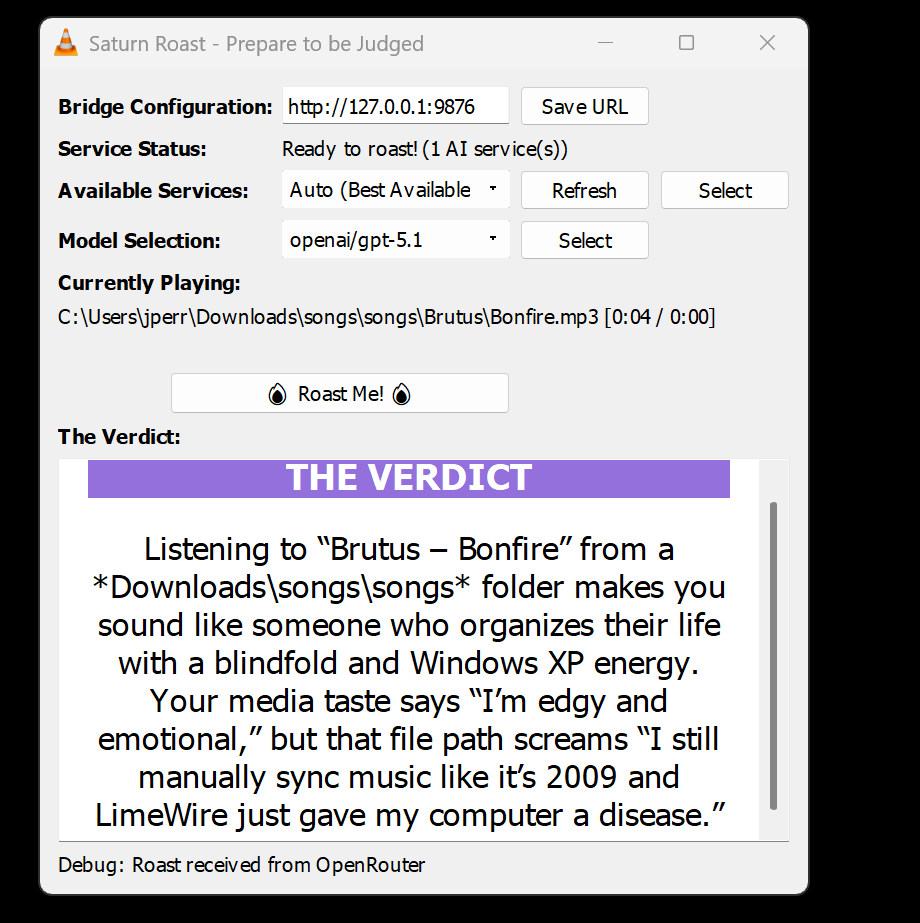
\includegraphics[width=0.75\textwidth]{figures/vlc-roast.png}
\caption{The Saturn Roast extension running inside VLC. The user selects a discovered service, clicks ``Roast Me!,'' and receives a short comedic roast of their media choices. No chat interface, model selector, or AI terminology is visible.}
\label{fig:vlc-roast}
\end{figure}

\section{Saturn Router: AI at the Network Infrastructure Layer}
\label{sec:router-implementation}

The VLC extension demonstrated that Saturn works in a consumer application.
The next question: could Saturn operate at the network level, embedded in the device that defines the network?
If Saturn runs on a router alongside DHCP and DNS, every device that joins the network gains AI access the same way it gains an IP address.

\subsection{Architecture and Technology Choices}

I structured the router implementation\footnote{\url{https://github.com/jperrello/Saturn/tree/main/saturn-router}} in three layers: a Rust binary managing the Saturn protocol, an OpenWRT integration layer embedding it into the router's service framework, and a LuCI web interface for browser-based administration.

The target hardware --- a GL.iNet GL-MT300N-V2 travel router with a MIPS32 processor and 128~MB of RAM --- cannot run a Python interpreter, so I made the choice to go with Rust. I scoped the build to this single router model; the binary cross-compiles to \texttt{mipsel-unknown-linux-musl} (a Rust Tier~3 target) using a Docker-based toolchain with soft-float musl and nightly \texttt{-Zbuild-std}.
Musl and MIPS32 constrained every dependency: \texttt{rustls} over \texttt{native-tls}, \texttt{attohttpc} over \texttt{reqwest} for a smaller binary, and aggressive size flags (\texttt{opt-level = "z"}, LTO, \texttt{panic = "abort"}).
Service registration uses the \texttt{mdns-sd} crate, a third independent mDNS library distinct from Python's \texttt{zeroconf} and JavaScript's \texttt{multicast-dns}.

The binary runs an event loop that ticks every 100 milliseconds: it health-checks upstream AI endpoints, rotates ephemeral credentials on schedule, and registers or unregisters the mDNS service based on backend availability.

I integrated the binary into OpenWRT using platform-native tooling: a \texttt{procd} init script manages process lifecycle with per-service JSON configuration files (permissions set to \texttt{600}), auto-downloading the binary from GitHub Releases if missing. A UCI schema exposes Saturn through the same \texttt{uci set}/\texttt{uci commit} workflow administrators use for firewall rules and DHCP. The LuCI web layer adds field validation, dynamic form visibility, and live status badges under the ``Services'' menu alongside DHCP and DNS.

Figure~\ref{fig:luci-config} shows the LuCI configuration page with its status badges.

\begin{figure}[H]
\centering
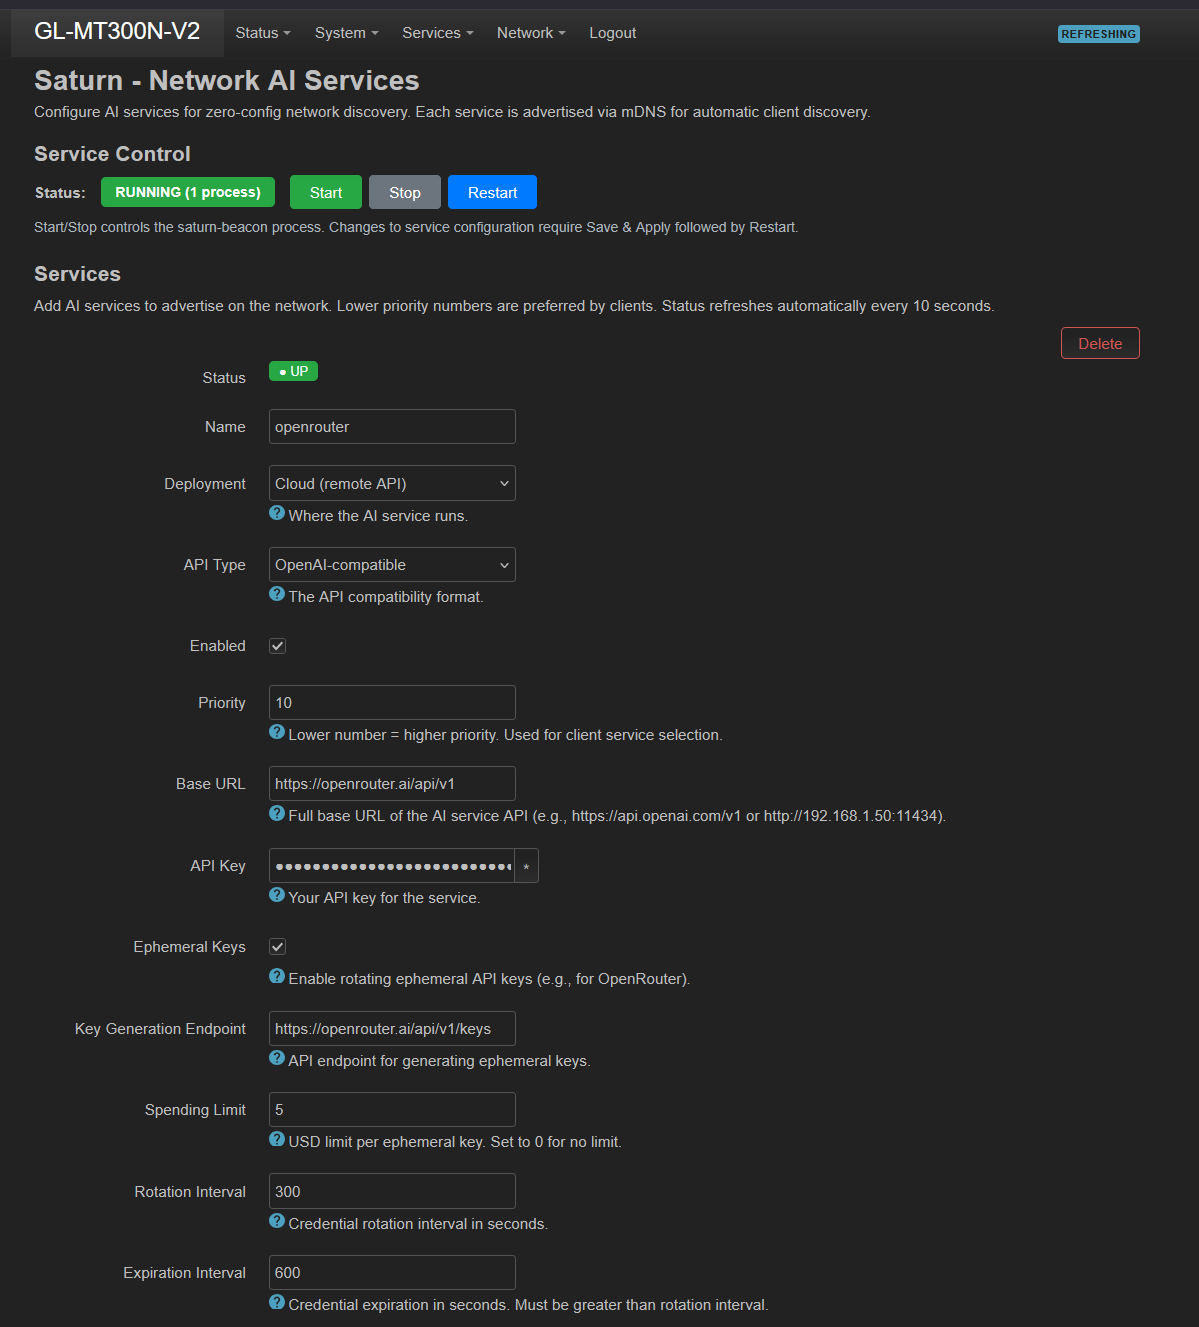
\includegraphics[width=0.85\textwidth]{figures/luci-config.png}
\caption{The Saturn configuration page in LuCI. Each service shows its name, deployment type, upstream endpoint, and a live status badge. Administrators manage Saturn through the same interface they use for DHCP and firewall rules.}
\label{fig:luci-config}
\end{figure}

\section{OpenCode: Saturn in an AI Coding Agent}
\label{sec:opencode-implementation}

While the VLC extension proved Saturn works in a non-AI application, neither it nor the router tests whether Saturn can handle a coding agent asking a model to edit three files, run a shell command, inspect the output, and continue the conversation --- all over a single streaming connection. OpenCode, an open-source terminal-based coding agent built by Anomaly, demands exactly this.
I forked OpenCode because Saturn requires runtime provider registration, a capability its static loader system does not support. The fork adds one capability --- dynamic provider discovery --- without modifying OpenCode's core routing, session management, or rendering. I integrated \texttt{ai-sdk-provider-saturn}\footnote{\url{https://github.com/jperrello/Saturn/tree/main/ai-sdk-provider-saturn}} as a bundled provider.

\subsection{Integration and Dynamic Registration}

I extended OpenCode's existing \texttt{CUSTOM\_LOADERS} provider system rather than forking its core abstractions.
The integration adds a \texttt{saturn} loader entry that creates a discovery instance with a three-second timeout, fetches \texttt{/v1/models} from all discovered services, and registers each model as a dynamic provider.
I touched twelve files across four packages but modified none of OpenCode's core abstractions. Confining changes to the loader layer forced the dynamic registration workaround described below.

Dynamic registration is the central challenge. OpenCode assumes the model set is fixed at startup, but Saturn models appear and disappear at runtime as services come online or fail. I bridged this gap with two callbacks: \texttt{onServiceDiscovered} fetches models from new services and calls \texttt{registerDynamic()}, while \texttt{onServiceRemoved} verifies the removal and calls \texttt{unregisterDynamic()}. Both callbacks emit events on instance-scoped and process-wide buses, updating model selectors in real time. The cost is that any component holding a model reference must tolerate that reference becoming invalid between ticks --- a stale reference fails silently rather than routing to a valid backend. I enforced invalidation through the event bus rather than polling.

Figure~\ref{fig:opencode-saturn} shows the model selector populated with Saturn-discovered models.

\begin{figure}[H]
\centering
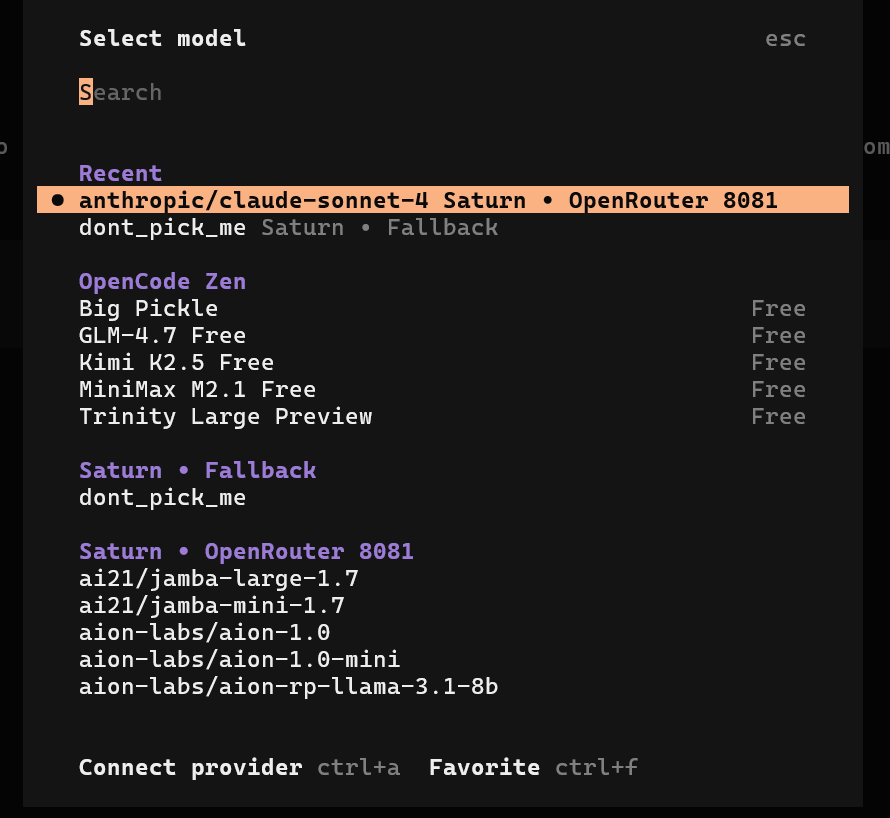
\includegraphics[width=0.85\textwidth]{figures/opencode-saturn.png}
\caption{OpenCode's model selector showing Saturn-discovered models. Each entry is prefixed with its service name (e.g., \texttt{saturn:office/gpt-4o}), populated at runtime through mDNS discovery with no user configuration.}
\label{fig:opencode-saturn}
\end{figure}

Integrating Saturn surfaced six bugs, three critical, and every critical bug traced to the same root cause: the host application assumed providers are configured at startup, not discovered at runtime. The simplest was a \texttt{finishReason} format mismatch: OpenCode expected AI SDK v2's plain string format (\texttt{"stop"}), but Saturn's provider returns v3 objects, fixed by one line of type normalization. Without a \texttt{toolCalling} capability flag, the agent lost the functionality that justified this implementation: OpenCode serialized function calls as plain text instead of invoking the tool-calling protocol, so the agent could chat but could not edit files or run commands; setting \texttt{toolcall: true} in the dynamic registration restored full agentic behavior. The most disruptive bug required the ugliest fix: Bun's default HTTP timeout killed long-running streaming requests, and because Bun provides no per-request timeout override, I monkey-patched \texttt{globalThis.fetch} to disable timeouts during streaming calls.

A concrete session illustrates the integration end-to-end. A developer launches OpenCode-Saturn in a project directory. The Saturn loader discovers two services, fetches their model lists, and populates the selector---the developer sees entries like \texttt{saturn:\allowbreak{}office/\allowbreak{}gpt-4o} without configuring any provider. The developer asks the agent to refactor a function; the agent streams a response while invoking file-edit and shell tools through the standard tool-calling protocol. If the office service goes down mid-session, failover reroutes to the same model on another service or sends an error if none available.

\section{Summary}
\label{sec:impl-summary}

Table~\ref{tab:impl-summary} summarizes the three implementations. Beyond these and the two SDK packages described above, I built two additional integrations: an Open WebUI plugin\footnote{\url{https://github.com/jperrello/Saturn/blob/main/owui_saturn.py}} (one uploaded file replaces per-backend configuration) and an MCP server\footnote{\url{https://github.com/jperrello/Saturn/tree/main/saturn-mcp}} (one JSON config entry exposes Saturn discovery as tools for AI coding assistants). Together, these seven artifacts span three languages and four mDNS libraries: VLC (Lua/Python, \texttt{dns-sd}), the router (Rust, \texttt{mdns-sd}), OpenCode, Open WebUI, and the MCP server (TypeScript/Python, \texttt{multicast-dns} and \texttt{zeroconf}).

\begin{table}[ht]
\centering
\small
\begin{tabular}{p{2.8cm} p{2.0cm} p{2.2cm} p{5.5cm}}
\hline
\textbf{Implementation} & \textbf{Language} & \textbf{mDNS Library} & \textbf{What It Demonstrates} \\
\hline
VLC Extension & Lua / Python & macOS \texttt{dns-sd} CLI & AI in a non-AI-native consumer application via bridge pattern \\
Saturn Router & Rust & \texttt{mdns-sd} crate & AI provisioning at the network infrastructure layer on constrained hardware \\
OpenCode Fork & TypeScript & \texttt{multicast-\allowbreak{}dns} npm & Full agentic AI workflow with tool calling, streaming, and dynamic discovery \\
\hline
\end{tabular}
\caption{Three Saturn implementations demonstrating progressive scope expansion. Each uses a different mDNS library, supporting argument~\argref{A10}: seven consumers across three languages and four mDNS libraries interoperate on \texttt{\_saturn.\_tcp.local.} with no bridging layer.}
\label{tab:impl-summary}
\end{table}

Each implementation answered a question left open by the previous one. Together they span the range from media players to network infrastructure to AI coding agents. Chapter~\ref{ch:evaluation} evaluates what these implementations demonstrate against the claims advanced in Chapter~\ref{ch:introduction}.


\chapter{Evaluation}
\label{ch:evaluation}

The Introduction advanced two claims: that zero-configuration protocols can provision AI services (\argref{C1}), and that network-level provisioning reduces total configuration effort (\argref{C2}). This chapter evaluates both. I assess \argref{C1} through an implementation census and protocol analysis, and \argref{C2} through a cognitive walkthrough following the methodology of Wharton et al.~\cite{wharton1994walkthrough}. The security trade-offs of broadcast discovery and a usability critique against Nielsen's heuristics~\cite{nielsen1994heuristics} receive their treatment in Chapter~\ref{ch:discussion}. The chapter closes with threats to validity. Both evaluations are analytical rather than empirical --- Saturn has no user base, no production deployment, and no institutional partner willing to run a field study --- and analytical methods are appropriate for a system at this stage because they evaluate design properties without requiring participants.

%----------------------------------------------------------------------
\section{C1: Zero-Configuration AI Provisioning Is Feasible}
\label{sec:eval-c1}

\argref{C1} asserts that mDNS/DNS-SD can provision AI services without end-user configuration. I decompose \argref{C1} into three requirements that together constitute an existence proof of feasibility, tracing the lifecycle of a zero-configuration AI connection. A service must first be \emph{found} without user input (R1). The discovery must then yield \emph{enough information} to connect (R2). Different implementations must agree on what they found, without sharing code (R3). If a service can be discovered, connected to, and consumed by independent clients, then zero-configuration provisioning is feasible.

\subsection{Results}

\paragraph{R1:}
Six implementations discover Saturn services through standard mDNS and DNS-SD queries on the \texttt{\_saturn.\_tcp.local.} service type. None requires a user-supplied URL, API key, or configuration file (\argref{A3}). The Python package, Rust router (Section~\ref{sec:router-implementation}), VLC extension, Open WebUI plugin, MCP server, and AI SDK provider each use their own mDNS library (\argref{A7}). The protocol, not my code, is what they share. This result connects directly to the access equity motivation from Chapter~\ref{ch:introduction}: if discovery requires no credentials and no configuration, then anyone on the network can use AI services regardless of whether they have a cloud provider account or a credit card.

\paragraph{R2:}
The TXT record schema (Section~\ref{sec:txt-schema}) carries everything a client needs to connect: endpoint URL, backend protocol, service priority, and hosting context (\argref{A8}). I tested this sufficiency against three backends with fundamentally different authentication models: Ollama requires none, DeepInfra uses a static JWT, and OpenRouter rotates ephemeral keys (\argref{A9}). All three work through the same schema with no out-of-band configuration necessary. This result matters beyond the protocol: schema sufficiency means any developer can integrate AI into an application without learning a provider's authentication model, billing API, or SDK. The schema carries that knowledge so the developer does not have to.

\paragraph{R3}
Seven consumers span three languages and four mDNS libraries (\argref{A10}): Python's \texttt{zeroconf}, Rust's \texttt{mdns-sd}, TypeScript's \texttt{multicast-dns}, and the macOS \texttt{dns-sd} CLI. No shared Saturn-specific code bridges them (\argref{A2}). Each parses standard DNS-SD TXT records independently. This is the result I find most telling: interoperability emerges from the protocol specification, not from a reference implementation I could have designed to make the numbers look good.

%----------------------------------------------------------------------
\section{C2: Reduced Configuration Effort}
\label{sec:eval-c2}

\argref{C2} asserts that Saturn reduces total configuration effort compared to per-user manual setup. I evaluate \argref{C2} using a cognitive walkthrough~\cite{wharton1994walkthrough}, counting discrete configuration actions each persona must perform to reach a single completion criterion: \emph{an end user on the network uses an AI-powered feature in an application.}

I define three personas that reflect Saturn's role model:

\begin{itemize}
  \item \textbf{Sysadmin} --- provisions the AI service and makes it available on the network.
  \item \textbf{App Developer} --- integrates AI capabilities into an application.
  \item \textbf{End User} --- consumes AI features through the developer's application.
\end{itemize}

Two conditions are compared. In the \emph{traditional} condition, the sysadmin obtains an API key from a cloud provider and distributes it to developers, who configure their applications with the key and expose AI features to end users, who create accounts and provide payment credentials. In the \emph{Saturn} condition, the sysadmin runs a Saturn beacon that advertises the service via mDNS; developers call \texttt{discover()} instead of configuring keys and URLs; end users do nothing.

The walkthrough scripts are implemented as annotated Python files in the project repository (\texttt{cog\_walkthrough/}), where each configuration action corresponds to a documented step. Step-counting optimizes for reproducibility and structural comparison: any reviewer following the same scripts arrives at the same counts. It sacrifices time measurement and cognitive difficulty weighting --- a limitation I address in Section~\ref{sec:eval-threats}. I chose a cognitive walkthrough over a user study because the relevant comparison is structural and because Saturn has no deployed user base from which to recruit participants.

\subsection{Results}

Table~\ref{tab:eval-cog} reports step counts per persona under each condition (\argref{A11}).

\begin{table}[ht]
\centering
\caption{Cognitive Walkthrough Step Counts by Persona}
\label{tab:eval-cog}
\begin{tabular}{l r r r}
\hline
\textbf{Persona} & \textbf{Traditional} & \textbf{Saturn} & \textbf{Change} \\
\hline
Sysadmin & 12 & 14 & +2 (+17\%) \\
App Developer & 19 & 4 & $-$15 ($-$79\%) \\
End User & 7 & 0 & $-$7 ($-$100\%) \\
\hline
\textbf{Total (1+1+1)} & \textbf{38} & \textbf{18} & $-$\textbf{20 ($-$53\%)} \\
\hline
\end{tabular}
\end{table}

The sysadmin does slightly more work: two additional steps to run a beacon process alongside the API key setup (\argref{CA3}). That is the cost. The payoff is stark. The app developer drops from nineteen steps to four, a 79\% reduction, because Saturn eliminates billing integration, key management, and endpoint configuration entirely (\argref{A12}). The end user drops to zero. No account creation, no payment credentials, no setup of any kind (\argref{A13}).

With one persona of each role, total steps drop from 38 to 18, a 53\% reduction. The reduction grows with scale because Saturn's formula has no $M$ term --- end users perform zero steps regardless of count (\argref{A14}):

\begin{align*}
\text{Traditional} &= 12 + 19N + 7M \\
\text{Saturn} &= 14 + 4N + 0M
\end{align*}

At $N = 10$ developers and $M = 100$ end users, this yields a 94\% reduction (902 vs.\ 54 steps).

The reduction is structural, not incremental: Saturn eliminates the entire billing and payment integration stack because the sysadmin's beacon already carries the credentials. Complexity centralizes in one administrator rather than scattering across $N$ developers and $M$ users. That is the core of \argref{C2}, and the step counts bear it out: 53\% reduction at minimum scale, 94\% at moderate scale. The reduction is not free --- the sysadmin absorbs two additional steps. But step counts treat all steps as equal, which they are not. Creating an API provider account is harder than running \texttt{pip install saturn}. I return to this limitation in Section~\ref{sec:eval-threats}.

%----------------------------------------------------------------------
\section{Threats to Validity}
\label{sec:eval-threats}

Three methodological threats constrain these conclusions. First, the three-persona model simplifies organizational reality. Roles overlap: a developer who also administers infrastructure would alter the per-persona step counts, though the structural elimination of billing and credential management persists regardless of role boundaries. Second, the cognitive walkthrough counts discrete actions but does not measure wall-clock time, error rates, or subjective difficulty. The identified steps --- package installation, service discovery, API calls --- are structurally simpler than traditional provisioning, but the methodology cannot confirm that they require less cognitive effort. Third, I, a single author, developed all seven service consumers and performed the walkthrough and the heuristic inspection reported in Section~\ref{sec:usability-critique}. Familiarity with Saturn’s architecture may consolidate multi-step processes, undercounting the friction a naive user would encounter. The executable Python walkthrough scripts provide a baseline for independent review, but single-author bias remains the most significant validity threat. Independent replication by external developers is required to robustly validate the feasibility and usability claims.



\chapter{Discussion}
\label{ch:discussion}

I believe Saturn's most immediate implication concerns institutional AI provisioning.  Bassignana et al.~\cite{bassignana2025aigap} documented the consequence of the not providing AI services to students --- students from lower socioeconomic backgrounds use AI tools less frequently and benefit less from them. Gabriel~\cite{gabriel2024educational} observed the same disparity in educational outcomes. Saturn introduces a third option: an institution deploys a Saturn beacon and funds a token budget with a cloud provider; every device that joins the network discovers the service automatically, and students pay nothing upfront. The institution pays only for tokens consumed, not seats licensed.

Shared token provisioning is not without risk. A budget split across an entire campus invites resource exhaustion: a small number of heavy users could drain funds intended for thousands. Institutions would need usage caps, per-student quotas, or tiered access policies. These are governance mechanisms Saturn does not provide and fall outside the protocol's scope. I raise this not to diminish the scenario but to acknowledge that provisioning AI as a shared resource introduces allocation problems that shared printers never faced, because inference costs scale with usage in ways that printer toner does not.

Saturn's contribution to AI democratization is structural, not incremental. Costa et al.~\cite{costa2024democratization} identified accessibility and usability as the two core dimensions of AI democratization --- the ability to reach AI tools without financial or technical barriers, and the effort required to operate them once reached. The cognitive walkthrough (\argref{A13}) found that Saturn reduces end-user configuration from seven steps to zero, suggesting progress on both dimensions: no financial barrier because the institution funds the token budget, and no usability friction because discovery is automatic. Whether Saturn fully satisfies Costa et al.'s criteria requires empirical validation with real users, but eliminating all end-user steps is a stronger signal than reducing them would be.

The passive discovery model is what I find most compelling about Saturn's potential. The current subscription model requires users to commit money before evaluating whether AI is useful to them. A user on a Saturn-enabled network encounters AI capabilities through applications that consume them automatically. The user may not even recognize that AI is involved --- they simply notice that their media player now translates subtitles, or their note-taking app now summarizes documents. That invisibility lowers the threshold for first contact with AI services and could bring inference to people who would never have sought it out. But invisibility cuts both ways. If users consume AI-generated output without knowing it, they lose the opportunity to evaluate its reliability, question its biases, or opt out. Applications that integrate Saturn bear a transparency obligation the protocol itself does not enforce.

\section{Security Trade-offs of Broadcast Discovery}
\label{sec:security-tradeoffs}

Saturn deliberately trades verification for accessibility. Requiring per-device authentication would reintroduce the credential burden Saturn exists to eliminate, so I chose to document and bound the exposure instead. The question is whether that trade-off is defensible --- whether the security surface of broadcast discovery is understood well enough to manage.

\subsection{What Saturn Exposes}

Saturn's TXT records broadcast eleven metadata fields to every device on the local network segment. In the base configuration --- backend and clients on the same network --- none contain credential material. Fields like \texttt{api\_base} and \texttt{api\_type} reveal the endpoint URL and backend protocol, but neither is a secret. Cloud deployments add exactly one credential field: \texttt{ephemeral\_key}, a time-limited API key with a ten-minute maximum lifetime and five-minute rotation interval (Section~\ref{sec:ephemeral-keys}). This is the only secret Saturn broadcasts, and it is short-lived by design. All fields are visible to any device on the local segment --- mDNS-SD traffic reaches every machine on the network by design (Section~\ref{sec:mdns-dnssd}).

Static API keys carry three high-severity threats (\argref{A5}). A stolen key enables spoofing with no time bound because it authenticates the bearer indefinitely. Static keys provide no temporal binding, making session attribution difficult and repudiation easy. Ephemeral credentials expire in ten minutes, limiting the spoofing window to a single rotation cycle. They rotate on a fixed schedule, providing the temporal binding that addresses repudiation. A leaked ephemeral key grants access for at most one cycle. Three medium-severity threats replace the three high-severity ones, all requiring LAN proximity: an attacker on the local network can observe the ephemeral key from mDNS traffic (information disclosure), use that key for up to ten minutes (tampering), or register a rogue \texttt{\_saturn.\_tcp.local.} service to redirect clients (service-level spoofing). Static API keys are exploitable from anywhere on the internet; Saturn's threats require physical or logical presence on the network segment.

The secret leakage data from Meli et al.~\cite{meli2019secrets} makes this comparison concrete. Most leaked API keys are never revoked, and the best automated scanners catch only a fraction of leaks (\argref{A16}). The static key lifecycle fails because keys persist until someone actively removes them, and the evidence shows removal rarely happens. Saturn's ephemeral model sidesteps this failure class: keys expire after ten minutes regardless of whether anyone detects a leak. A Saturn key committed to a public repository would be dead before any scanner could find it. I do not claim that ephemeral credentials make Saturn secure in an enterprise sense. They convert unbounded, internet-scale threats into bounded, LAN-scoped ones --- and the resulting threat surface is documented in the mDNS security literature that Kaiser and Waldvogel~\cite{kaiser2014privacy} established.

\subsection{AP Isolation}

One deployment constraint directly undermines the campus scenario that motivated this work (\argref{A17}). Enterprise and institutional WiFi networks commonly enable AP isolation, which blocks multicast traffic between wireless clients. I confirmed in  that both eduroam and UCSC-Guest block mDNS. Saturn services advertised on these networks are invisible to client devices. This is an infrastructure policy decision and it means Saturn cannot operate on the networks where the access equity motivation is strongest. Saturn works on home networks, office LANs, and lab environments where multicast flows freely. It fails on institutional networks with client isolation.

%----------------------------------------------------------------------
\section{Usability Critique}
\label{sec:usability-critique}

The preceding sections interpret Saturn's functional results and security surface. A single-author inspection against Nielsen's ten usability heuristics~\cite{nielsen1994heuristics}, applied across the three-persona model from Section~\ref{sec:eval-c2}, reveals what those results mean for the people who would use the system.

Saturn's strongest usability property is recognition over recall (\argref{A18}). Discovered services appear as a list with endpoint URLs, backend types, and priority rankings already resolved. Automated assignment of addresses, ports, and failover priorities prevents the configuration slips that manual provisioning invites: malformed URLs, stale endpoints, mismatched ports. This is the mechanism through which Saturn delivers the step reductions the cognitive walkthrough measured. The developer's four remaining steps succeed because none requires recalled knowledge about a provider's API surface.

Three weaknesses emerge, each tied to a design trade-off. First, Saturn's invisibility to end users creates a control gap. Administrators and developers can manipulate service discovery, but end users cannot override misconfigured priorities that degrade their experience. The zero-step end-user experience comes at the cost of zero end-user agency. Second, Saturn's terminology --- ``beacon,'' ``proxy,'' ``service type'' --- matches protocol semantics but diverges from administrator mental models, where ``model endpoint'' is the natural concept. This gap matters less for protocol correctness than for adoption: administrators who cannot map Saturn's vocabulary to their existing infrastructure concepts will resist deploying it. Third, and most critically, Saturn lacks failure diagnostics. When discovery fails, the client reports a generic ``service not available'' error that does not distinguish between AP isolation blocking multicast, no beacon running, or a misconfigured beacon. Nielsen's error recovery heuristic requires that error messages identify the problem and suggest corrective action; Saturn does neither. The AP isolation problem from above compounds this weakness: the most common deployment failure --- institutional WiFi blocking multicast --- produces the least informative error.

\section{Future Work}
\label{sec:future-work}

I chose mDNS-only discovery because it requires no infrastructure beyond the network itself --- no central registry, no DNS records to configure, no server to maintain. That purity is also the protocol's sharpest constraint. The AP isolation barrier (\argref{B5}) demands a hybrid discovery architecture: pairing mDNS with a lightweight unicast fallback that advertises Saturn services via a well-known HTTPS endpoint. The concrete flow would be: a client on eduroam queries \texttt{\_saturn.\_tcp} via mDNS, receives no response, then falls back to \texttt{https://saturn.ucsc.edu/.well-known/saturn} for endpoint metadata. That fallback reintroduces a configuration dependency --- someone must provision and maintain the HTTPS endpoint --- but the dependency falls on the administrator, not the end user. The design goal is to preserve Saturn's zero-configuration property for the student while accepting that institutional networks require institutional infrastructure. Success means a student on eduroam discovers a Saturn service as seamlessly as one on a home network.

Empirical user studies would complement the analytical evaluation. I would run a controlled experiment comparing configuration time and error rates between Saturn and traditional API key provisioning, across participants with varying technical backgrounds, to test whether the step reductions from the cognitive walkthrough translate to real usability gains. Carmona-Galindo et al.~\cite{carmona2025hsi} documented how generative AI adoption varies across student populations at Hispanic-serving institutions; I would prioritize that context to directly test Saturn's potential to reduce the access disparities that Bassignana et al.~\cite{bassignana2025aigap} identified.

Finally, Kaiser and Waldvogel's privacy-preserving mDNS-SD extensions~\cite{kaiser2014efficient} offer a path toward confidential discovery. Their privacy sockets and pairing mechanisms maintain backward compatibility with standard mDNS while encrypting service advertisements to authorized clients. Integrating these extensions would enable Saturn deployments in shared workspaces or medical facilities where broadcasting AI service availability raises privacy concerns the current protocol does not address.

The gap between AI's falling inference costs and its persistent access barriers is a protocol problem, not a cost problem. The infrastructure to close that gap has existed for over a decade; what remained was the evidence that it generalizes and the honesty about where it breaks. If the hybrid discovery and empirical validation work I have outlined succeed, the next generation of students will encounter AI as something the network simply provides.


\chapter{Conclusion}
\label{ch:conclusion}

This thesis asked whether AI services could be provisioned at the network level, discovered automatically and consumed without credentials or configuration. Saturn answers that question with a protocol, three implementations, and an analytical evaluation. The three implementations tested the protocol in different settings: a VLC media player extension brought AI into a consumer application that has never had it, a router firmware integration provisioned AI on a router, and an AI coding agent fork handled streaming tool calls and multi-turn conversation. The specification, not a reference implementation, carries the interoperability. Saturn's current reach is bounded by institutional WiFi's AP isolation, which blocks multicast discovery on the networks where access equity matters most. A hybrid architecture pairing mDNS with a unicast HTTPS fallback would extend Saturn to these environments, and controlled user studies would test whether the analytical step reductions translate to real usability gains. The gap between AI's collapsing inference costs and its persistent access barriers is a provisioning problem. Saturn demonstrates that existing protocols mDNS/DNS-SD can apply to AI services in order to make them more accessibile and require less configuration then current alternatives



% ============================================================
% APPENDICES
% ============================================================
\appendix

\chapter{Generative AI in Thesis Development}
\label{app:ai-methodology}

This appendix will explain the use of LLMs in the completion of this thesis, and during the development of Saturn. This section, along with the Generative AI acknowledgement are entirely hand written me. Every other section of this thesis is the output of a LLM, specifically, Anthropic's Claude series of models. The code for Saturn and the thesis are visible on their respective Github repositories and is entirely the output of these large language models. The methods behind generating this code is described below. These methods are my best attempt to steer LLMs to be more reflective of my true intentions, design patterns, and beliefs. This system provided me with an agent that could serve as an agentic advisor, going beyond the guidance of one hour weekly sessions with the primary research advisor. This agentic workflow is effective at designing a thesis, retrieving facts and claims from memory, and correcting itself. This system hopes to provide a level of sophistication for papers that use generative AI in their creation.

\section{Design Fictions}

Design fictions are an existing practice of creating fictional scenarios where a non-existing idea becomes real, with the goal of creating speculative and provocative discussions about the idea. Design fictions have been used in debate for decades, however they provide a unique advantage with LLMs to create specification documents for a system. Design fictions provide a working example of an idea that can be reverse engineered by an LLM. The design fictions for Saturn can be found in the fiction directory of the Saturn Github repository. They follow the story of two fictional characters, Derek and Mira, and a fictional corporation: Megalink. Derek's role was a software engineer and self-proclaimed ``home network wizard,'' meant to reflect a technically proficient integrator of Saturn who has configured Saturn on their network. The Megalink corporation is the company that created the system that would ultimately become Saturn. Mira symbolizes a non-technical user. She is the sister of Derick who visits and uses Saturn on Derick's network to generate AI captions on a fictional photo app. She didn't need to pay for anything or configure settings, she just joined Derek's network and she had new features that were not present before. Later, a new character, Jordan, was created to inspire the beacon system. Jordan was a developer who had leaked his company's API key from a Saturn server. Beacons were created to provision short lived keys on the network that are deleted after a short window. As said before, when a LLM reads this design fiction, it isn't interpreted as speculation, it instead becomes a vision that can be broken down into specs. The three characters provide the LLM with examples of who in the real world would use Saturn. There is an understanding that the end user (Mira) and the programer who configures Saturn on their network (Derek) require different types of documentation and tools. These design fictions lead to the initial specifications for the Saturn protocol and first implementations.

\section{Documentation Website}

During development of Saturn, a human and agent facing documentation website was created with the intent to be referenced to a coding agent in future context. Myself, or any other person could visit the website and use it as a reference for their coding agents, as it served as the main knowledgebase for Saturn. In fact, the documentation site has a llms.txt file specifically designed to guide AI agents. The documentation is split across three different sections: the user guide, the integrator guide, and an integrations page. The user page provides a high level overview of the system, and a short guide for discovering Saturn services on the network. I purposefully tried to avoid technical jargon such as mDNS, TXT records, and endpoints. This page can therefore serve as an introduction to new users of the system, or it can be injected into the prompt for an agent for context about Saturn. The integrator guide provides the technical overview of Saturn and is meant to be read by developers and network administrators. This page includes how to configure a custom Saturn service, which endpoints were required, and Saturn SDK guides. This page provided basic context to agents implementing Saturn. The last page showcased integrations of Saturn in hopes of growing popularity for the protocol. If I designed a page that could prove how easy it is to implement Saturn as a protocol, it could become more popular and therefore standardized. Coding agents could be fed this site as context to understand how similar platforms have integrated Saturn in the past. Integrators or coding agents could submit their personal integrations of Saturn on a form on this page, which then become Github Issues for the website. This website was frequently used as a source of knowledge that was fed to an agent upon fresh work sessions. Without it, Saturn would need to be explained every session, risking the loss of implementation details and worse context for the agent. This webpage later served as an initial source of memory for the Moons system, which will be described later in the appendix.

\section{Integrations into Various Applications}

An important goal of Saturn was to create multiple interoperable technical prototypes built around the protocol \_saturn.\_tcp.local, demonstrating that widespread adoption was feasible. Initially Saturn was integrated into the chat based AI applications OpenWebUI and Jan, later moving to the coding agent OpenCode. All these platforms were natively based in AI, meaning some readers or developers may disregard Saturn entirely if they are working on projects or apps that are not AI native. Adam and Joey believed that Saturn made AI possible in apps that were not AI native, and to prove this, Joey created a VLC extension that roasted a user based off of what media was playing. There was no chat, and no mention of AI whatsoever. Developing these integrations could have each been a master project on their own. However, Joey took advantage of coding agents to develop them faster instead. I was able to integrate to these platforms faster because they would often have thorough documentation or source code on the web to reference to a coding agent. This had a snowball effect where the more integrations got built, the more examples of Saturn could be given as context to future agent sessions.

\section{Serve Role as a ``Robotic'' Advisor}

Joey and Adam met once a week on an hourly basis to discuss Saturn. Outside of that hour, the AskUserQuestion tool incorporated into Claude Code would assist in taking notes for writing the thesis paper. I actively engaged with Claude Code to arrive at different claims for the thesis, organize background work, and create an evaluation plan by chatting, and answering questions. Initially, the agent wrote all of its memory of Saturn and the interviews in a single markdown file. This file was disorganized, lacked technical depth, or misinterpreted information I would reference. The agent struggled to remember previous conversations the student would have, and it would have difficulty piecing together the repository, previous academic work, and the claims of the system. There needed to be a system that gave agents the same level of knowledge I had about Saturn, while providing the ability to hyperfocus on specific sections of the thesis depending on the focus of a work session.

\section{Moons}

Moons is the memory system that served as the knowledge base for all coding agents while I wrote the thesis. Moons did not exist while Saturn was being developed, only during the writing process of my thesis. The name ``moons'' comes from Saturn, the planet, notoriously having a lot of moons. Each individual moon can be thought of containing one small piece of information about the greater and more complex Saturn. Moons is a JSON file that points to different directories and markdown files in the moons directory. Each entry in this JSON file has the following fields:

\textbf{id:} the element of saturn that the current chunk is describing. Example: claim1, beacons, ai-sdk

\textbf{type:} this describes what role the id has in the saturn project. Example: claim1 has a type of claim, and beacons has a type of concept.

\textbf{Desc:} A short one sentence description of what the element is. Example: ephemeral-keys description reads ``Time-limited API credentials (10-min lifetime, 5-min rotation with overlap for zero-downtime transitions) distributed via mDNS TXT records and deleted on shutdown, paralleling Kerberos session-layer distribution. Implemented in Python (KeyManager with thread-safe locks) and Rust (full lifecycle with `Drop` impl), making the `leaked secret never removed' class (Meli 2019: 81\%) structurally impossible.''

\textbf{File:} reference to where a detailed markdown file of the concept is. These files contain a more detailed explanation of the ID, where to find the source files related to the ID, and why it matters in the project.

\textbf{Edges:} list of other ids and their relation to the current chunk

Example moon chunk:

\begin{verbatim}
{"id": "mdns", "type": "concept", "desc": "Link-local name resolution
(RFC 6762) via multicast to 224.0.0.251:5353 requiring no DNS server —
Saturn's protocol foundation, used identically to how Bonjour discovers
printers, AirPlay, and Chromecast. Key limitations: AP isolation blocks
multicast (confirmed on eduroam/UCSC-guest Jan 2026), passive
eavesdropping exposes all announcements, and 59% of device names leak
real user names.", "file": "concepts/mdns.md", "edges": [
    {"to": "claim-1", "rel": "supports"},
    {"to": "dns-sd", "rel": "related"},
    {"to": "ch2", "rel": "discussed_in"},
    {"to": "ch3", "rel": "discussed_in"}
]},
\end{verbatim}

The goal of moons is to create a knowledge graph for an agent. With moons, a conversation about Saturn is much easier because I could freely reference source material with my agent having a memory bank to reference. An example question would be: ``What have we discussed in claim 2 so far, is there anything I am forgetting to add?'' An agent can read the graph.json to find claim-2's id and trace all the details for claim-2 through markdown files. I, the human in the loop, could see if my agent is forgetting any information, or hallucinating the results and claims I previously made. A drawback to this strategy is that the graph.json has to be read in its entirety every time moons are mentioned. This drawback helps provide Claude with a high level understanding of all of the components of Saturn and how they all connect, but ultimately fills the context window with irrelevant information. My alternative option was to query the graph via a script, but this strategy proved to be even more inefficient as one read call is cheaper than multiple bash calls considering Saturn's graph.json was \textasciitilde563 lines. The agent also has to have knowledge of the moons system each session, and the only way to effectively provide the knowledge of moons existence is via an AGENTS.md file or a CLAUDE.md file. This ended up taking 20 lines in my CLAUDE.md file which is already a context burden for most systems, but proved to not have a noticeable effect for this thesis.

\begin{verbatim}
### Moons (Knowledge Base)
This project uses a structured knowledge graph called `moons/` to organize all
thesis context.

**Structure:**
- `moons/graph.json` — the map. Lightweight nodes with typed edges. Read this
FIRST to navigate.
- `moons/concepts/` — Saturn concepts (mDNS, DHCP, ephemeral keys, etc.)
- `moons/claims/` — the 3 thesis claims with evidence
- `moons/papers/` — distilled paper summaries with relevance to Saturn
- `moons/voice/` — user's personal perspective, design rationale, interview
notes
- `moons/code/` — code component analyses with line citations
- `moons/chapters/` — chapter planning and section status
- `moons/meta/` — advisor notes, timeline, project context

**How to use:**
1. Always `Read(moons/graph.json)` first. At ~500 lines it's cheap to read in
full and gives complete graph visibility — all nodes, edges, and types in one
shot. This holistic view is intentional: it surfaces connections you weren't
looking for.
2. Follow edges to specific content files only when you need depth.
3. After interviews or new information, update both the relevant content file
AND graph.json edges.
4. Keep graph.json lean — short descriptions, not full content. Depth lives in
the files.
5. `moons/query.py` exists as a human CLI convenience (`python moons/query.py
edges-to claim-3`).

**Moons is the workspace. thesis.tex is the submission.** Moons organizes
thinking; thesis.tex is the final output.
\end{verbatim}

I often discovered gaps of knowledge or evidence in Saturn by viewing the moons knowledgebase. I would notice certain chunks had less edges than I believed they should, leading me to discover I forgot to upload an implementation piece of Saturn to the thesis. Moons highlighted areas of Saturn that had the most evidence, and which areas needed more support or focus. Coding agents also had knowledge of how moons worked, meaning they could create interactive websites for visualizing Saturn's ideas.

\section{Finding Academic Papers}

Google announced Scholar Labs during the research phase of Saturn. Google Labs is a search engine that is powered by Gemini, and is developed like most chat bots; a user can query in natural language and the model will find academic papers related to that question. With the knowledge stored in moons, I could ask my agent to generate research questions for my thesis to be later sent to Scholar Labs. Once I had a result I would read the abstract, results, and figures of each paper before downloading and storing them inside the moon's knowledge base. The agent would always require approval for its integration of the paper, and this process was continuously iterated for finding more papers. The moon knowledge base grew as my own understanding and research behind Saturn grew.

\section{AI Contribution in the Evaluation Section}

The second claim in the evaluation section of this thesis was that Saturn ultimately provided less cognitive overhead than traditional API configuration methods. To prove this, my strategy was to perform a cognitive walkthrough, where I documented a series of steps in order to convey the workload required to accomplish each configuration setup. The initial goal was for an agent to autonomously count all the steps with the MCP server Playwright in isolated Docker containers. This ended up failing as the system was unreliable and difficult for me to verify. Perhaps with the invention of OpenClaw I overlooked an entirely agentic system. Instead, I opted for a different approach that relied on my previous design fiction's three different audiences for Saturn. There are people who configure Saturn on the network, app developers incorporating Saturn, and end users who consume the ai services. I first performed a 100\% human-written cognitive walkthrough of creating an API key on Openrouter and placing it in an environment variable file. These were shared steps that both a system with and without Saturn needed to take. After this initial cognitive walkthrough, I wrote python scripts from the design fiction's multiple perspectives:

\begin{itemize}
\item An app developer using saturn's python package to send a query to an api endpoint
\item An app developer using the traditional method of querying an api endpoint (including Stripe billing)
\item The cognitive walkthrough for a sys admin distributing api keys to their team
\item The cognitive walkthrough of a sys admin configuring a saturn beacon on their network without using the saturn python package
\item The cognitive walkthrough of a sys admin configuring a saturn beacon on their network using the saturn python package
\item An end user using an app with saturn on their network
\item An end user using an app that uses AI without saturn
\end{itemize}

Note: These python scripts are as minimal as possible and try to avoid excessive features. The end user scripts contain no runnable code, rather just a docstring of the walkthrough this fictional person went through.

\section{Academic Writing Skill}

LLMs played a pivotal role in generating the text written in the thesis document. I created Moons to solve the problem of giving the agent memory of Saturn, and I utilized the AskUserQuestion tool to conduct self-guided interviews on my thoughts and claims for the thesis. Still, I faced a consistent problem: AI agents continuously failed to write what I considered to be captivating and well-written academic papers. The papers themselves are long and flood context, not including the knowledge required to remember what arguments and evidence are required when writing the paper. Even with the moon's knowledge base, it was impossible to one-shot a well written thesis in a singular prompt. Dividing the thesis into context-manageable sections wasn't effective either as the agent would often repeat information referenced in other sections of the thesis. I also believe AI writing to be subpar and lacking substance, with most of its output content following the same structure that eventually becomes a glaring pattern. Additionally, models had the tendency to scatter knowledge with no cohesion. To solve this problem I created the academic-writing skill. An agent will invoke this skill when the user directly mentions it or the description matches the problem the user is asking the agent to solve. For the academic-writing skill my description read:

\begin{quote}
``Use this skill whenever writing prose, essays, academic content, reports, or any long-form written output, even if the user doesn't explicitly mention writing quality. Trigger for any drafting, revising, or editing of written sections --- including when the user pastes text and asks for feedback.''
\end{quote}

The skill's body includes general writing skills that I personally believed to be best practice and reflected how I wanted the thesis to be written. The rules of writing were divided into the following sections: Concreteness, Reader-Centered Writing, Dialogic Framing, Structure, and Rigor. The body also included a core workflow of drafting, evaluating, revising, and presenting the revision. These rules and the workflow were written to be generalizable enough that they could be applied to any area of my thesis. I wanted individual sections of my thesis to have specific rules and guidelines for writing, so markdown files were created for rules on that specific section of the thesis. The main skill body directed the agent to read the markdown file associated with the section it was writing. Now, agents could invoke this skill to write or make changes to specific sections (like the abstract or evaluation) of the thesis. It had the rules to generally follow, but also the rules for writing specific areas. There is no mention of Saturn itself in this skill, as I wanted the agents to understand these rules applied to all types of academic writing and not Saturn in isolation.

\section{AI Detection Ralph Loop}

Ralph loops were invented by Geoffrey Huntley and they allow a user to run fresh agent sessions with the same prompt infinitely. A simple Ralph loop looks like this:

\begin{verbatim}
while :; do cat PROMPT.md | claude-code ; done
\end{verbatim}

This trick allows agents to correct themselves and complete a long repetitive task autonomously. While I was writing my thesis, I noticed that no matter how many interviews or evidence there was in moons, the agent would still write vapid claims or fail to see the thesis as a whole piece of work, not individual sections. Initially, I planned to run Sapling, an ai detection software, inside a Ralph loop so an agent can receive a score and try to minimize the score for the next pass. Adam was strongly opposed to this idea, as there was no clear goal or structure behind beating the score. An agent could essentially game the system and not actually improve the quality of writing. So, Adam and Joey read through sections of the thesis and transcribed to an agent what they believed to be common mistakes and blunders the agent was making when writing. Claude then organized this transcription into ``academic-advisor-notes.md.'' These notes served as guidelines that a subagent was given to grade my thesis. After this session, I designed a new Ralph loop. The Ralph loop begins with an agent reading notes from the previous Ralph session, the academic advisor notes, and the moons graph. Then, this agent spawns a subagent that reads the content of the thesis and grades based on the guidelines of Adam and I. This read-only subagent returns the grade back to the main agent with specific sections annotated as needing more correction than others. The main agent uses the knowledge it previously read about, and the academic-writing skill, to rewrite the thesis. After the thesis is finished, the agent takes notes of the score the thesis received before edits and the changes it took to write those sections better. These notes have the goal of steering future agents towards some writing strategies and away from others. If the previous Ralph iteration made major changes but the score decreases in the next session, that future agent knows to avoid the tips that the old agent left notes for. This Ralph loop process ultimately led to the creation of the first thesis draft that I eventually tweaked section by section.

\section{Structured Arguments Skill}

The structured arguments skill was a skill used for an agent to organize my claims, evidence, reasoning, arguments, etc in a format that was modeled after Belcak et al. (2025) ``Small Language Models are the Future of Agentic AI.'' This paper labels every claim, argument, and counter-argument with short IDs and cross-references them throughout. This was a formatting skill but ultimately made the thesis easier to follow while eliminating my burden of manually labelling.



% ============================================================
% BIBLIOGRAPHY
% ============================================================
\singlespacing
\setlength{\bibsep}{\baselineskip}
\bibliographystyle{plain}
\bibliography{references}

\end{document}
